\subsection{Command Line Interface (CLI)}\label{subsec:cli}
LuRaCs is primarily operated through the GUI but it also provides a terminal-based command line interface, allowing for controlling detectors without a GUI. This may be useful if remote measurements or measurements run on a Raspberry Pi is attached to a drone. This mode shares most of the same commands as the GUI Console with the exception of visualisation tools.

This mode is started by running LuRaCs in a terminal with the \texttt{--headless} flag.

\begin{figure}[H]
    \centering
    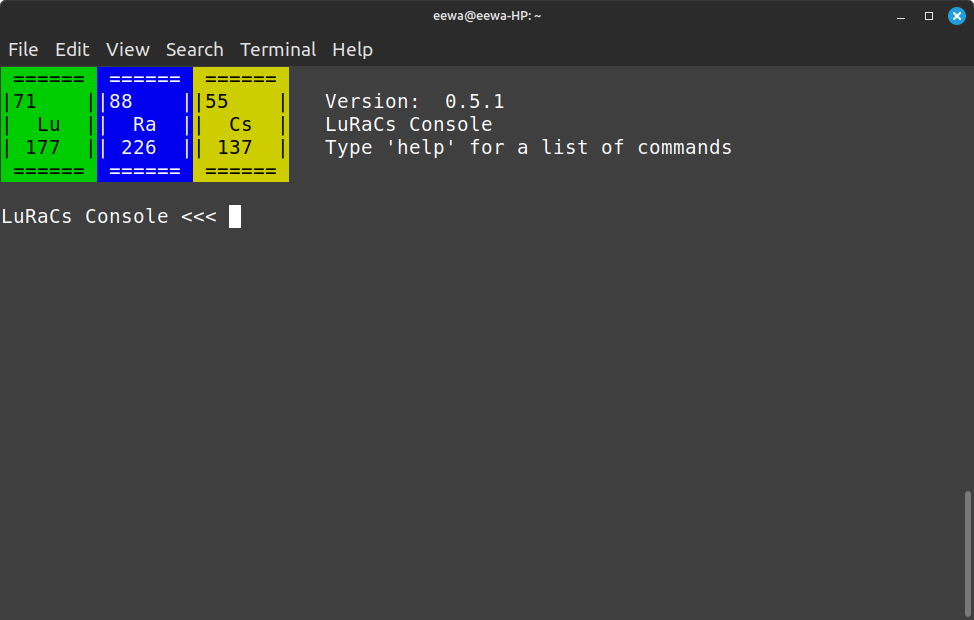
\includegraphics[width = .8\linewidth]{images/interface/cli.png}
    \caption{LuRaCs command line interface in terminal mode.}
    \label{fig:cli}
\end{figure}

\begin{figure}[H]
    \centering
    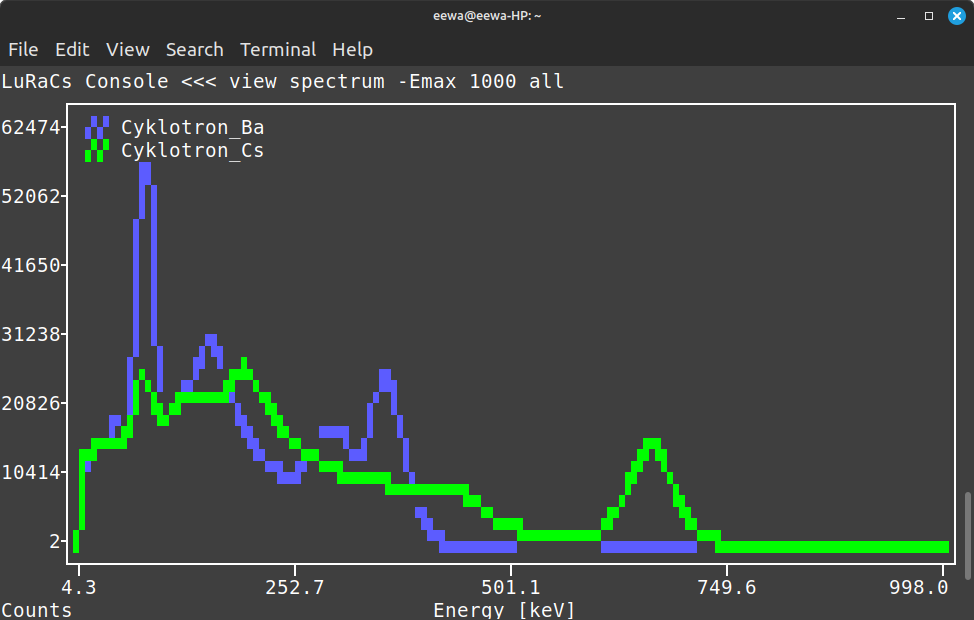
\includegraphics[width = .8\linewidth]{images/interface/cli_spectrum.png}
    \caption{Two spectra viewed through the command line using the command \texttt{view spectrum -Emax 1000 all}. The \texttt{-Emax 1000} flag limits the x-axis to $< 1000$ keV.}
    \label{fig:cli_spectrum}
\end{figure}

%---------------------------------------------------------------
% Command Reference
% ----------------------------------------------------------------

\begin{longtable}{>{\ttfamily}p{0.38\textwidth} p{0.55\textwidth}}
    \caption{Command-line interface command reference.}
    \label{tab:command-reference} \\

    \hline
    \textnormal{\textbf{Command}} &
    \textnormal{\textbf{Description}} \\
    \hline
    \endfirsthead

    \multicolumn{2}{c}%
    {\tablename\ \thetable{} -- continued from previous page} \\
    \hline
    \textnormal{\textbf{Command}} &
    \textnormal{\textbf{Description}} \\
    \hline
    \endhead

    \hline
    \multicolumn{2}{r}{Continued on next page} \\
    \endfoot

    \hline
    \endlastfoot

    % ============================================================
    % General
    % ============================================================

    \multicolumn{2}{l}{\textbf{General}} \\
    \texttt{help} &
        Display the available commands and their descriptions. \\

    \texttt{clear} &
        Clear the console and return the application to start. \\

    \texttt{exit}, \texttt{quit}, \texttt{shutdown} &
        Exit the application. \\

    \hline

    % ============================================================
    % Device Management
    % ============================================================

    \multicolumn{2}{l}{\textbf{Device Management}} \\

    \texttt{device scan usb} &
        Scan for connected USB devices. \\

    \texttt{device scan ble} &
        Scan for nearby Bluetooth Low Energy devices. \\

    \texttt{device connect usb <device>} &
        Connect to a USB device matching the specified name. \\

    \texttt{device connect ble <device1> [device2 ...]} &
        Connect to one or more Bluetooth Low Energy devices. \\

    \texttt{device disconnect <device>} &
        Disconnect the specified device. \\

    \texttt{device disconnect all} &
        Disconnect all connected devices. \\

    \hline

    % ============================================================
    % Resource Listing
    % ============================================================

    \multicolumn{2}{l}{\textbf{Resource Listing}} \\

    \texttt{list devices} &
        Display all connected devices. \\

    \texttt{list spectra} &
        Display all loaded spectra. \\

    \texttt{list spectrogram} &
        Display all loaded spectrograms. \\

    \texttt{list rois} &
        Display all loaded regions of interest. \\

    \hline

    % ============================================================
    % Indexes
    % ============================================================

    \multicolumn{2}{l}{\textbf{Indexes}} \\

    \texttt{index spectrum} &
        Display indexed spectrum files. \\

    \texttt{index spectrogram} &
        Display indexed spectrogram files. \\

    \texttt{index roi} &
        Display indexed ROI files. \\

    \hline

    % ============================================================
    % Viewing
    % ============================================================

    \multicolumn{2}{l}{\textbf{Viewing Data}} \\

    \texttt{view spectrum <name>} &
        Display the specified spectrum. The spectrum can be selected by name
        or by its index in the loaded spectrum list. \\

    \texttt{view spectrum -n <name>} &
        Specify the spectrum to display by name. \\

    \texttt{view spectrum all} &
        Display all loaded spectra on the same plot. \\

    \texttt{view spectrum -A} &
        Display all loaded spectra on the same plot. \\

    \texttt{view spectrum -Emin <energy>} &
        Set the lower energy limit of the displayed spectrum, in keV. \\

    \texttt{view spectrum -Emax <energy>} &
        Set the upper energy limit of the displayed spectrum, in keV. \\

    \texttt{view spectrum -cps} &
        Display the spectrum as counts per second (CPS) instead of total
        counts. \\

    \texttt{view spectrum -log} &
        Display the spectrum using the logarithmic scaling. \\

    \texttt{view spectrum -bkgSub} &
        Display the background-subtracted spectrum, if the spectrum has a background. \\

    \texttt{view rois} &
        Display the currently loaded regions of interest. \\

    \texttt{view log} &
        Display recent application log entries. \\

    \hline

    % ============================================================
    % ROI
    % ============================================================

    \multicolumn{2}{l}{\textbf{ROI Management}} \\

    \texttt{roi <lower> <upper>} &
        Add a region of interest between the specified lower and upper
        bounds. \\

    \texttt{roi -c} &
        Clear all regions of interest. \\

    \hline

    % ============================================================
    % Spectrogram
    % ============================================================

    \multicolumn{2}{l}{\textbf{Spectrogram Management}} \\

    \texttt{spectrogram start <device>} &
        Start a spectrogram for the specified device. \\

    \texttt{spectrogram start all} &
        Start spectrograms for all connected devices. \\

    \texttt{spectrogram pause <name>} &
        Pause the specified spectrogram. \\

    \texttt{spectrogram pause all} &
        Pause all running spectrograms. \\

    \texttt{spectrogram unpause <name>} &
        Resume the specified spectrogram. \\

    \texttt{spectrogram unpause all} &
        Resume all paused spectrograms. \\

    \texttt{spectrogram load <path>} &
        Load a spectrogram from the specified file. \\

    \texttt{spectrogram unload <name>} &
        Unload the specified spectrogram. \\

    \texttt{spectrogram unload all} &
        Unload all loaded spectrograms. \\

    \texttt{-n <name>} &
        Specify a custom name when starting a spectrogram. \\

    \texttt{-i <seconds>} &
        Set the spectrogram save interval. Default: $1$ second. \\

    \texttt{-c <count>} &
        Set the number of spectra to concatenate before saving.
        Default: $1$. \\

    \hline

    % ============================================================
    % Maps
    % ============================================================

    \multicolumn{2}{l}{\textbf{Map Management}} \\

    \texttt{map url <https-URL>} &
        Load an online map from the specified HTTPS URL. \\

    \texttt{map file <path>} &
        Load a local offline map from a PMTiles file. \\

    \hline

    % ============================================================
    % Monitoring
    % ============================================================

    \multicolumn{2}{l}{\textbf{Monitoring}} \\

    \texttt{watch} &
        Continuously display live information from connected devices.
        Press \texttt{Ctrl+C} to stop. \\

    \hline

    % ============================================================
    % Automation
    % ============================================================

    \multicolumn{2}{l}{\textbf{Automation}} \\

    \texttt{exec <script-file>} &
        Execute commands from a script file. Empty lines and lines
        beginning with \texttt{\#} are ignored. \\

\end{longtable}